\documentclass[11pt]{beamer}

\logo{\includegraphics[width=.55in]{figures/logoBCAM.png}} 
\newcommand{\nologo}{\setbeamertemplate{logo}{}}

\usepackage{framed}
\usepackage{longtable,booktabs}
\usepackage{caption}
\usepackage{xcolor,colortbl}
\usepackage{animate}

%\usebackgroundtemplate{\includegraphics[width=\paperwidth,height=\paperheight]{light-grey-background.png}}

\setlength{\parskip}{10pt plus 1pt minus 1pt}

\definecolor{BCAMblue}{RGB}{5,102,181}
\definecolor{BCAMgrey}{RGB}{71,67,64}

\mode<presentation>
{
  \usetheme{default}
  \usecolortheme{seagull}
  \usefonttheme{professionalfonts}
  \setbeamercolor{math text}{fg=BCAMblue}
  \setbeamercolor{math text displayed}{fg=BCAMblue}
}

\makeatletter
\renewcommand\verbatim@font{\color{BCAMgrey}\normalfont\ttfamily}
\makeatletter

\everymath{\color{BCAMgrey}}

\useoutertheme{infolines}

\makeatletter
\setbeamertemplate{footline}
{
  \leavevmode%
  \hbox{%
  \begin{beamercolorbox}[wd=.333333\paperwidth,ht=2.25ex,dp=1ex,center]{author in head/foot}%
    \usebeamerfont{author in head/foot}\insertshortauthor~~\beamer@ifempty{\insertshortinstitute}{}{(\insertshortinstitute)}
  \end{beamercolorbox}%
  \begin{beamercolorbox}[wd=.333333\paperwidth,ht=2.25ex,dp=1ex,center]{title in head/foot}%
    \usebeamerfont{title in head/foot}\insertshorttitle
  \end{beamercolorbox}%
  \begin{beamercolorbox}[wd=.333333\paperwidth,ht=2.25ex,dp=1ex,right]{date in head/foot}%
    \usebeamerfont{date in head/foot}\insertshortdate{}\hspace*{2em}
    \insertframenumber/\inserttotalframenumber\hspace*{2ex}
  \end{beamercolorbox}}%
  \vskip0pt%
}
\makeatother


\setbeamertemplate{navigation symbols}{}


\usepackage{xcolor, url}
\makeatletter
\renewcommand\verbatim@font{\color{BCAMgrey}\normalfont\ttfamily}
\makeatletter

\everymath{\color{BCAMgrey}}
\definecolor{WhiteSmoke}{rgb}{0.961,0.961,0.961}

\setbeamercolor{titlelike}{fg=BCAMblue,bg=WhiteSmoke} %
\setbeamercolor{title in sidebar}{fg=WhiteSmoke}      %
\setbeamercolor{author in sidebar}{fg=WhiteSmoke}     %
\setbeamercolor{framesubtitle}{fg=BCAMgrey}    

\setbeamercolor*{normal text}{fg=black,bg=white}
\setbeamercolor*{alerted text}{fg=BCAMblue}

%Include packages
\usepackage[spanish]{babel}
%\usepackage[T1]{fontenc}
\usepackage[latin1]{inputenc}
\usepackage{natbib}
\usepackage{amssymb}
\usepackage{amsthm}
\usepackage{amsmath}
\usepackage{hyperref}
\usepackage{graphics}
\usepackage{graphicx}

\newcommand{\comment}[1]{}

\beamertemplatetheoremsunnumbered  %This supresses theorem numbers

\renewcommand{\thesection}{\arabic{section}}
\renewcommand{\thesubsection}{\arabic{section}.\arabic{subsection}}
%
\renewcommand{\thetable}{\arabic{table}}
\renewcommand{\thefigure}{\arabic{figure}}
%
\newcommand{\bfa}{\mbox{\boldmath $a$}}
\newcommand{\bfd}{\mbox{\boldmath $d$}}
\newcommand{\bfe}{\mbox{\boldmath $e$}}
\newcommand{\bfu}{\mbox{\boldmath $u$}}
\newcommand{\bfs}{\mbox{\boldmath $s$}}
\newcommand{\bfv}{\mbox{\boldmath $v$}}
\newcommand{\bfx}{\mbox{\boldmath $x$}}
\newcommand{\bfy}{\mbox{\boldmath $y$}}
\newcommand{\bfz}{\mbox{\boldmath $z$}}
\newcommand{\bfA}{\mbox{\boldmath $A$}}
\newcommand{\bfB}{\mbox{\boldmath $B$}}
\newcommand{\bfC}{\mbox{\boldmath $C$}}
\newcommand{\bfD}{\mbox{\boldmath $D$}}
\newcommand{\bfE}{\mbox{\boldmath $E$}}
\newcommand{\bfG}{\mbox{\boldmath $G$}}
\newcommand{\bfH}{\mbox{\boldmath $H$}}
\newcommand{\bfI}{\mbox{\boldmath $I$}}
\newcommand{\bfJ}{\mbox{\boldmath $J$}}
\newcommand{\bfL}{\mbox{\boldmath $L$}}
\newcommand{\bfM}{\mbox{\boldmath $M$}}
\newcommand{\bfP}{\mbox{\boldmath $P$}}
\newcommand{\bfQ}{\mbox{\boldmath $Q$}}
\newcommand{\bfR}{\mbox{\boldmath $R$}}
\newcommand{\bfT}{\mbox{\boldmath $T$}}
\newcommand{\bfU}{\mbox{\boldmath $U$}}
\newcommand{\bfV}{\mbox{\boldmath $V$}}
\newcommand{\bfW}{\mbox{\boldmath $W$}}
\newcommand{\bfY}{\mbox{\boldmath $Y$}}
\newcommand{\bfX}{\mbox{\boldmath $X$}}
\newcommand{\bfeta}{\mbox{\boldmath $\eta$}}
\newcommand{\bfbeta}{\mbox{\boldmath $\beta$}}
\newcommand{\bfalpha}{\mbox{\boldmath $\alpha$}}
\newcommand{\bfepsilon}{\mbox{\boldmath$\epsilon$}}
\newcommand{\bfmu}{\mbox{\boldmath $\mu$}}
\newcommand{\bfrho}{\mbox{\boldmath $\rho$}}
\newcommand{\bfgamma}{\mbox{\boldmath $\gamma$}}
\newcommand{\bfdelta}{\mbox{\boldmath$\delta$}}
\newcommand{\bfvarepsilon}{\mbox{\boldmath $\varepsilon$}}
\newcommand{\bfzero}{\mbox{\boldmath $0$}}

\newcommand{\bfMu}{\mbox{\boldmath $M$}}
\newcommand{\bftheta}{\mbox{\boldmath $\theta$}}
\newcommand{\bfTheta}{\mbox{\boldmath $\Theta$}}
\newcommand{\bfLambda}{\mbox{\boldmath $\Lambda$}}

\newcommand{\bfotimes}{\mbox{\boldmath $\otimes$}}
\newcommand{\bfone}{\mbox{\boldmath $1$}}
\newcommand{\bfnot}{\mbox{\boldmath $0$}}
\newcommand{\bfpsi}{\mbox{\boldmath $\psi$}}
\newcommand{\bfSigma}{\boldsymbol{\Sigma}}
\newcommand{\bfZ}{\boldsymbol{Z}}
\newcommand{\n}{\~{n}}
\newcommand{\ii}{\'{\i}}
\newcommand{\tR}{\mbox{\texttt{R~}}}

\newtheorem{lema}{Lema}[]

\usefonttheme[onlymath]{serif} 

 
\title[Introduction to P-splines]{Introduction to penalized splines}
\subtitle{3$^{\rm a}$ Jornada J\'ovenes Investigadores SEB}

\author[D.-J. Lee]{Dae-Jin Lee}


\institute[BCAM]{\large Basque Center for Applied Mathematics}
% - Use the \inst command only if there are several affiliations.
% - Keep it simple, no one is interested in your street address.

%
\date[{\bf JJSEB 3}]{\url{https://wp.bcamath.org/jjseb3}}


% \AtBeginSection[]
% {
%   \begin{frame}<beamer>{Outline}
%     \tableofcontents[currentsection]
%   \end{frame}
% }

\usepackage{Sweave}


\begin{document}
\input{JJSEB3-concordance}






\begin{frame}
  \titlepage
\end{frame}



% \begin{frame}[fragile]
% \frametitle{Internet Access}
% \Large
% 
% \textbf{NETWORK:}  \verb|BCAM_VISITOR| \\
% 
% \textbf{PASSWORD:} \verb|SaZLwZutY6|
% 
% \end{frame}

%\begin{frame}[plain,allowframebreaks]
\begin{frame}
\frametitle{Outline}
 %\footnotesize
  \tableofcontents
\end{frame}




\section[Introduction]{Introduction}


\begin{frame}
 \frametitle{From linear regression to penalized regression}
 	\framesubtitle{\quad Basics}
 \vspace{-.cm}
 
{\footnotesize
\begin{itemize}
\item Scatterplot of pairs $(\bfx_i,\bfy_i)$, $i=1,...,n$
\end{itemize}

\vspace{-.1cm}
\begin{minipage}[c]{.525\columnwidth}
\only<1>{
\begin{center}
%%%\animategraphics[autoplay,width=.9\textwidth,clip=true,trim = 10pt 25pt 0pt 50pt]{50}{gifs/aa}{0}{84}
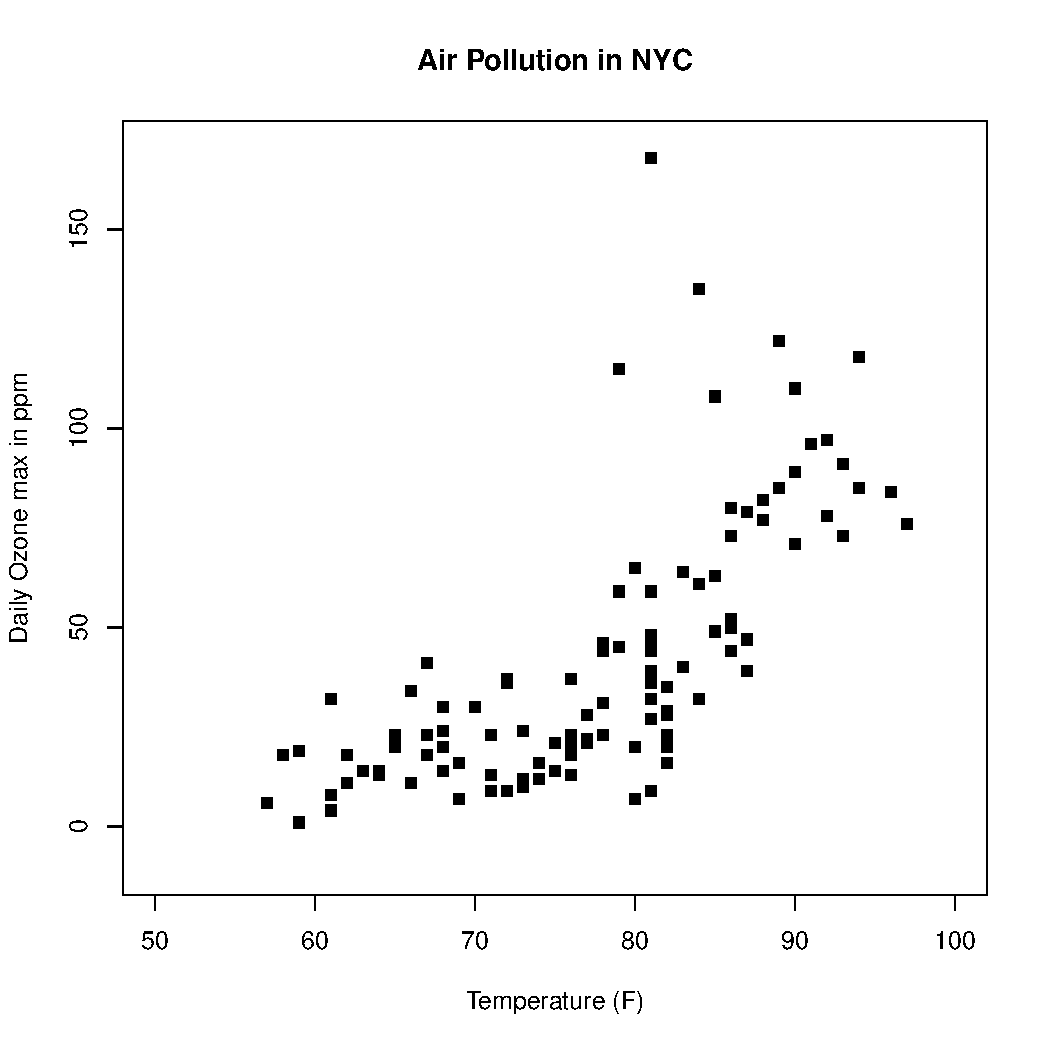
\includegraphics[width=.9\textwidth, height=.5\textheight,clip=true,trim = 0pt 15pt 0pt 10pt]{figures/fig0}
\end{center}
}
\only<2>{
\begin{center}
%%%\animategraphics[autoplay,width=.9\textwidth,clip=true,trim = 10pt 25pt 0pt 50pt]{50}{gifs/aa}{0}{84}
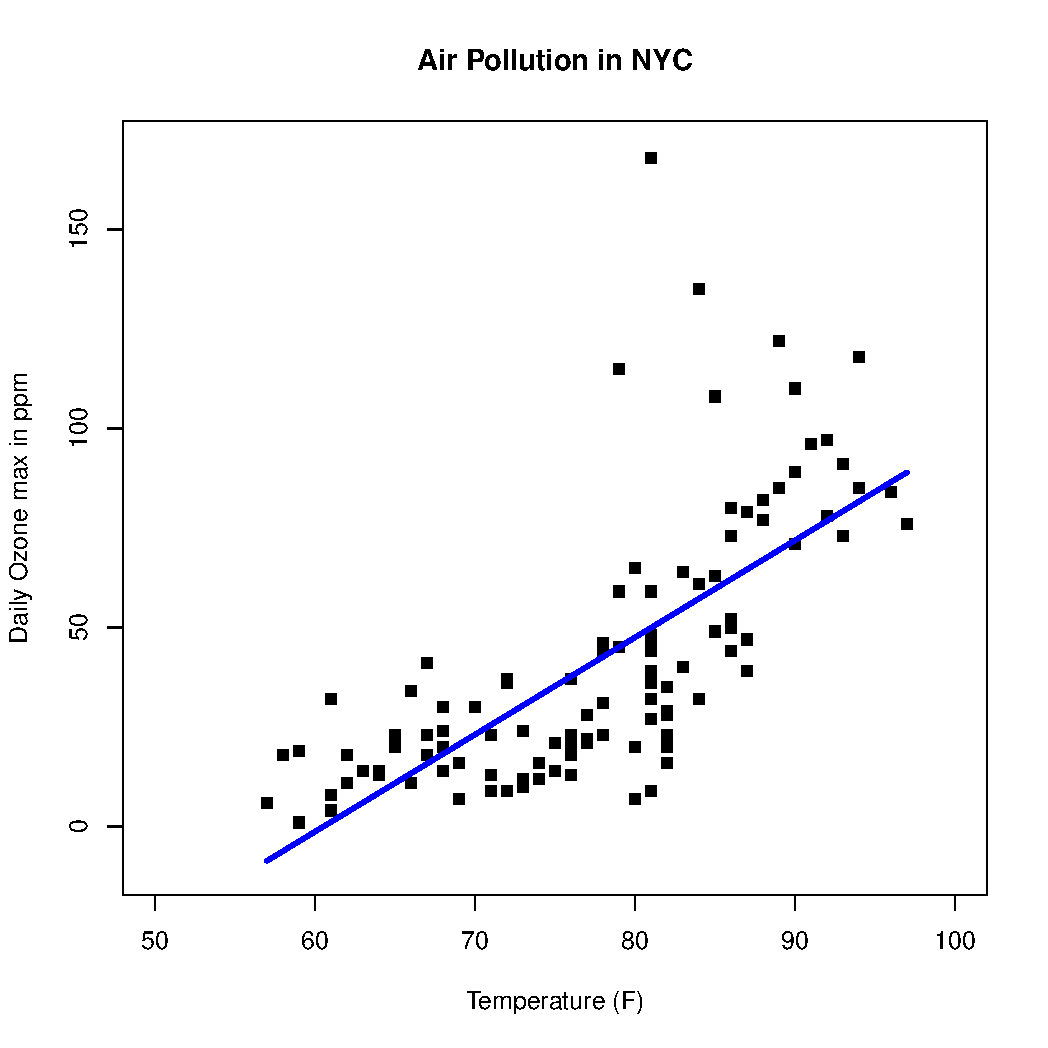
\includegraphics[width=.9\textwidth, height=.5\textheight, clip=true,trim = 0pt 15pt 0pt 10pt]{figures/fig1}
\end{center}
}
\end{minipage}
\begin{minipage}[c]{.43\columnwidth}
\begin{alertblock}{}
\begin{itemize}
\item \alert{Assumption:} straight line fits data well
%\item \alert{Equation:} \boxed{\bfy_i= \bfbeta_0 + \bfbeta_1 x_i + \bfepsilon_i} with $\mbox{E}[\bfepsilon_i]=0$ and $\mbox{Var}[\bfepsilon_i]=\sigma^2$\medskip
\item[]\qquad {\boxed{\mbox{E}[\bfy_i|\bfx_i]= \bfbeta_0 + \bfbeta_1 x_i}}
% \item \alert{In matrix form:} \quad $\hat \bfy = \bfX\hat \bfbeta$
\medskip
\item Minimize least squares criteria
{\scriptsize
\[
% \min \sum_{i=1}^n (\bfy_i - \hat \bfy_i)^2 
\min \|\bfy - \hat\bfy \|^2 
\]
}
\vspace{-.25cm}
\end{itemize}
\end{alertblock}
\end{minipage}
% \pause
}

\vfill

\vfill

\end{frame}




\begin{frame}
 \frametitle{From linear regression to penalized regression}
 	\framesubtitle{\quad Beyond linear regression}
 \vspace{.0cm}
{\footnotesize
\begin{itemize}
\item Linear fit is {\color{red}\bf too simple} and not always OK

\item {\bf Alternative:} use higher degree powers of $\bfx$, with $\bfX = [~\bfone_n , \bfx_i , \bfx_i^2 , ... , \bfx_i^{p}~]$ 

\item Columns of $\bfX$ are \alert{basis functions} (polynomial regression)
\end{itemize}
\vspace{-.35cm}
\begin{center}
%%%\animategraphics[autoplay,width=.9\textwidth,clip=true,trim = 10pt 25pt 0pt 50pt]{50}{gifs/aa}{0}{84}
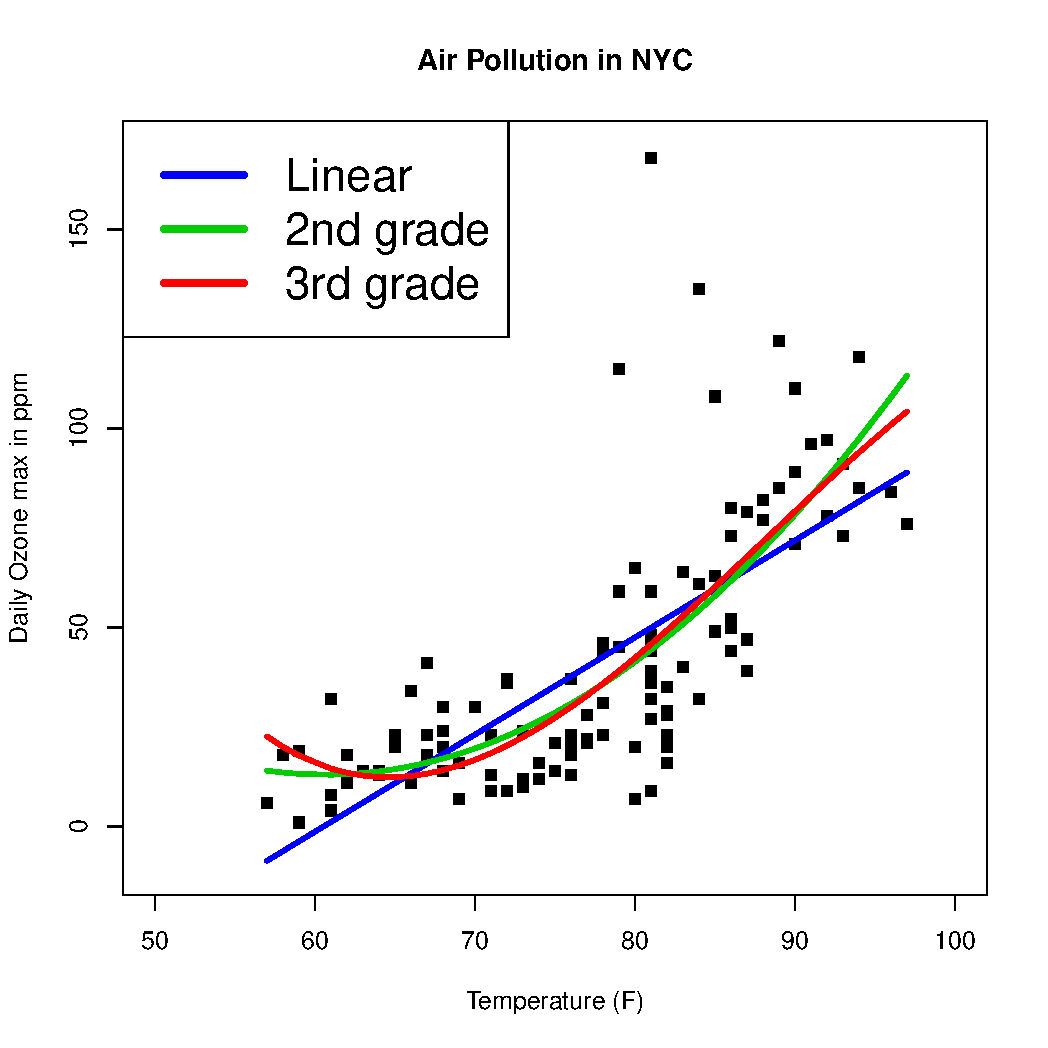
\includegraphics[width=.55\textwidth, height=.5\textheight,clip=true,trim = 0pt 15pt 0pt 10pt]{figures/fig2}
\end{center}
\vspace{-.5cm}
\begin{itemize}
\item Same regression equations: $\hat\bfbeta = (\bfX^\prime\bfX)^{-1}\bfX'\bfy$
\end{itemize}
}

\vfill
\end{frame}







\begin{frame}
 \frametitle{From linear regression to penalized regression}
 	\framesubtitle{\quad non-parametric regression or smoothing}
 \vspace{-.20cm}
{\footnotesize
\begin{itemize}
\item Instead of simple linear regression, we can fit the model:
\[
\boxed{\mbox{E}[\bfy_i|\bfx_i]= f(\bfx)}
\]\vspace{-.25cm}
\item[]\quad where $f(\bfx)$ is an arbitrary \alert{smooth function} \medskip

\item The model is ``non-parametric'' in the sense of no distributional assumptions for the parameters as in a linear model (\alert{scatterplot smoothing}).\medskip

%\item Enormous literature in smoothing since late 80's (theoretical aspects on how much to smooth)

\item Wide variety of methods (since 80's):

\begin{itemize}
\item \footnotesize kernel smoothing, local linear methods, smoothing splines, etc ... ({\color{red}\bf out-of-fashion!})
\item \alert{Penalized regression splines} are getting popular
\begin{itemize}
\item \footnotesize combine a rich set of \alert{basis functions}, with a \alert{roughness penalty}
\end{itemize}
\end{itemize}
\end{itemize}
}


\vfill

\vfill

\end{frame}


%%%%%

\section{Splines, regression splines and Smoothing splines}
{\nologo
\begin{frame}
 \frametitle{Splines}
 \vspace{-.20cm}
{\footnotesize
\begin{itemize}[<+->]
\item {\it a $k$th order spline is a piecewise polynomial function of degree $k$, that is continuous
and has continuous derivatives of orders $1,...k-1$, at its knot points.}
\item {\it Formally, a function $f:\mathbb{R}\rightarrow\mathbb{R}$ is a $k$th order spline with knot points at $t_1< ... < t_m$, if}
 \begin{itemize}
 \item {\it $f$ is a polynomial of degree $k$ on each of the intervals $(-\infty,t_1],[t_1,t_2],...[t_m,\infty)$, and}
 \item  {\it $f^{(j)}$, the $j$th derivative of $f$, is continuous at $t_1,...,t_m$, for each $j= 0,1,...k-1$.}
  \end{itemize}
\item {\it By requiring continuous derivatives, we ensure that the resulting function is as smooth as possible.}
\item {\it We can obtain more flexible curves by increasing the degree of
the spline and/or by adding knots.}
\item {\it However, there is a tradeoff:}
\begin{itemize}
	\item {\it \footnotesize Few knots/low degree:  Resulting class of functions may be too
restrictive (bias).}
	\item {\it \footnotesize Many knots/high degree:  We run the risk of overfitting (variance).}
\end{itemize}
\end{itemize}

}


\vfill

\vfill

\end{frame}
}


{\nologo
\begin{frame}
 \frametitle{Splines (cont.)}
 \vspace{-.20cm}
{\footnotesize
\begin{itemize}[<+->]
\item {\it The most common case considered is $k= 3$,  i.e.,  that of {\bf cubic splines}.  These are piecewise cubic functions that are continuous, and have continuous first, and second derivatives.}
\item {\it How can we parametrize the set of a splines with knots at a given set of points $t_1,...t_m$
?  The most natural way is to use the {\bf truncated power basis}, $g_1,...g_{m+k+1}$, defined as}
$$
g_1(x) = 1,\quad g_2(x) = x,...,\quad g_{k+1}(x)=x^k,
$$ 
\vspace{-.2in}
$$
  g_{k+j+1}(x)= (x - t_j)^{k}_+,\quad j=1,...,m.
$$
where $x_+$ denote the positive part of $x$, i.e. $x_+ = \mbox{max}\{x,0\}$.

\item {\it These types of fixed-knot models are referred to as {\bf regression splines}}

\item {\it The truncated power basis are:}
 \begin{itemize}
  \item {\footnotesize \it Conceptually simple.}
  \item {\footnotesize \it Simpler models are nested inside it, leading to straightforward tests of null hypotheses.}
  \item {\footnotesize \it Computationally inefficient (singularity problems).}
 \end{itemize}  
\end{itemize}
}
\vfill

\vfill

\end{frame}
}

{\nologo
\begin{frame}
 \frametitle{Splines (cont.)}
 \vspace{-3.25cm}
\begin{center}
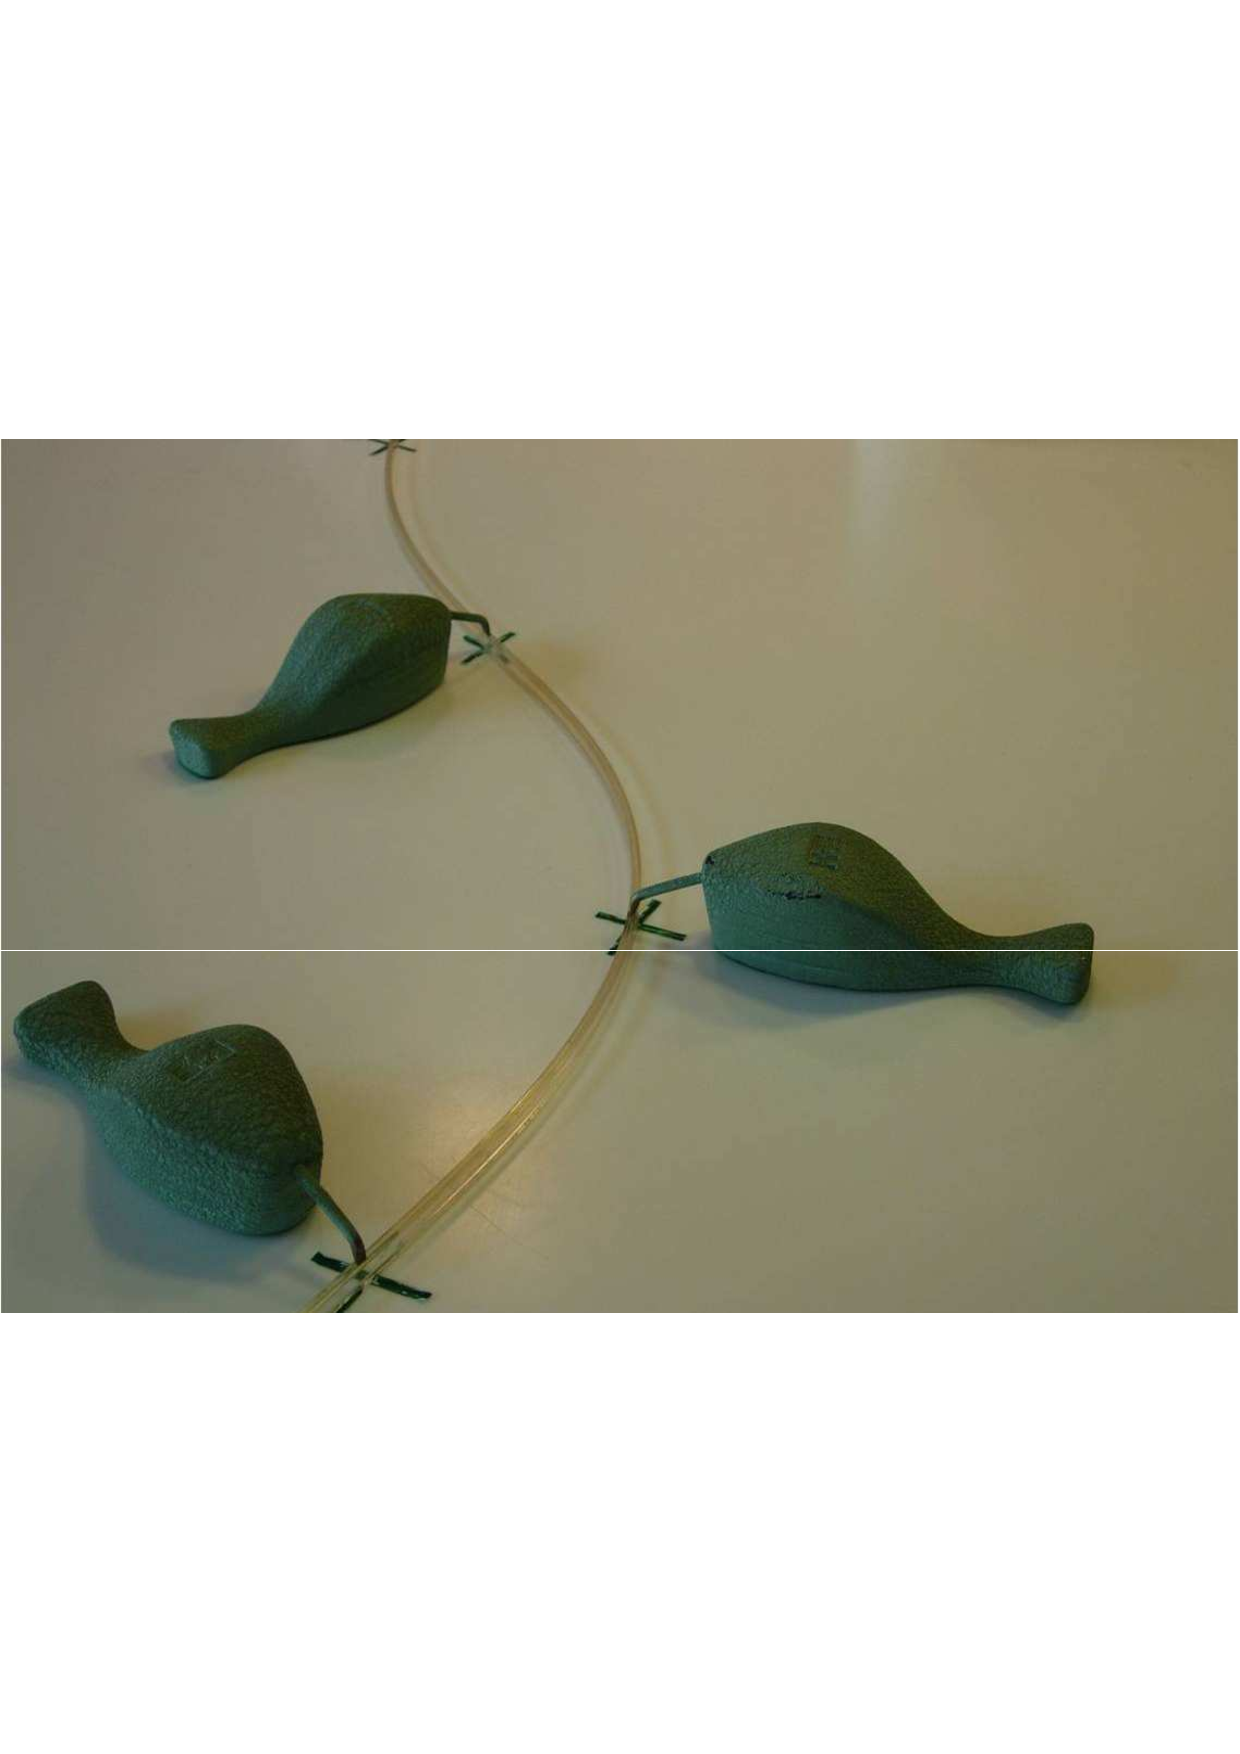
\includegraphics[scale=.8]{figures/spline22}
\end{center}
\vfill

\vfill

\end{frame}
}

{\nologo
\begin{frame}
 \frametitle{Splines (cont.)}
 \vspace{-.15cm}
\begin{center}
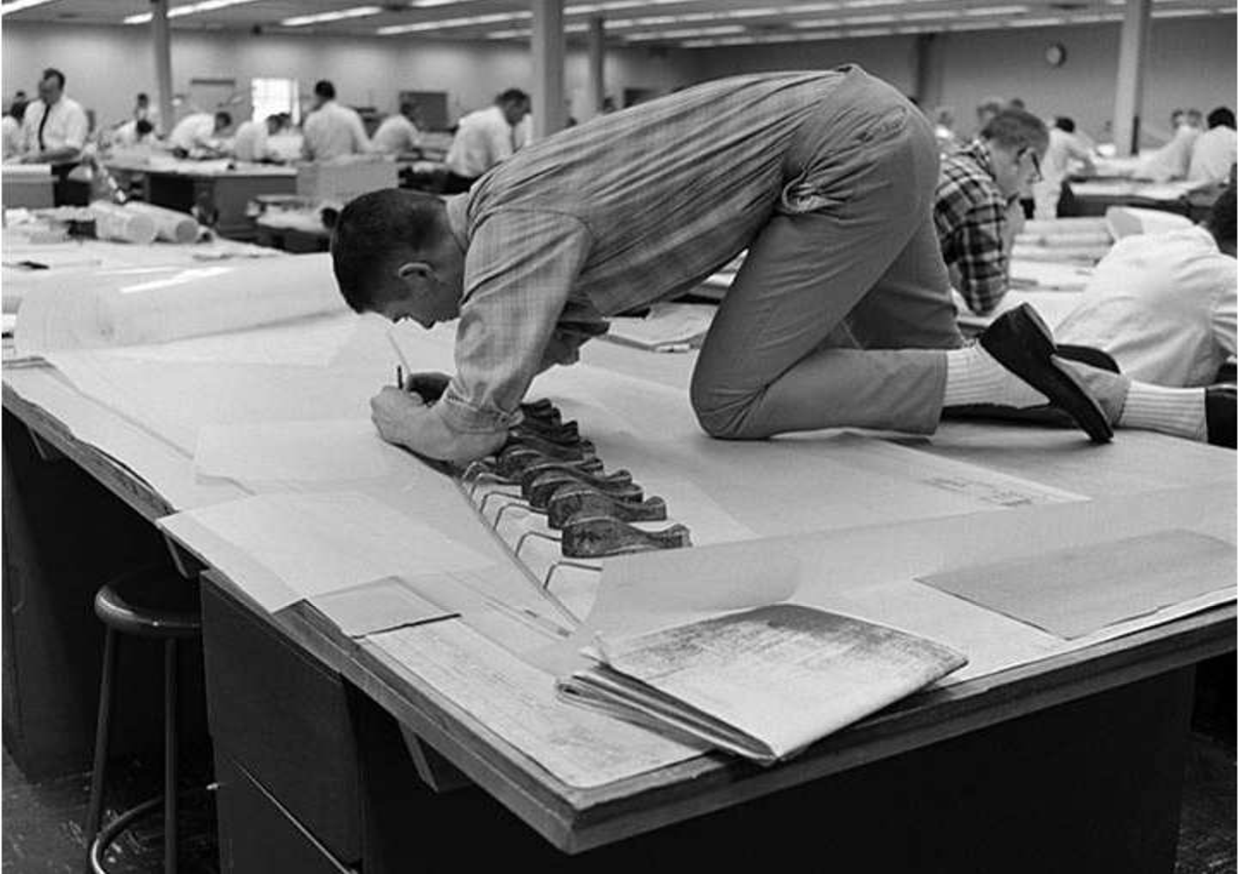
\includegraphics[scale=.8]{figures/spline1}
\end{center}
\vfill

\vfill

\end{frame}
}

\begin{frame}[fragile]
  \frametitle{Truncated power basis in \texttt{R}}

\centering
\begin{Schunk}
\begin{Sinput}
> tpoly<-function(x,t,p){
+ # p order truncated polynomials
+ B=NULL
+ for(i in 1:length(t)){
+ B=cbind(B,(x-t[i])^p*(x>t[i]))}
+ B
+ }
\end{Sinput}
\end{Schunk}
\end{frame}

{\nologo
\begin{frame}[fragile]
  \frametitle{Truncated power basis in \texttt{R}}

\begin{figure}
\centering
\includegraphics{JJSEB3-003}
\end{figure}
\end{frame}
}



{\nologo
\begin{frame}
 \frametitle{B-splines (de Boor, 1978)}
 \vspace{-.20cm}
{\footnotesize
\begin{itemize}%[<+->]
\item a much better computational choice, both for speed and numerical accuracy, is the B-spline
basis.
\item {\bf One linear B-spline} 
 \begin{itemize}
  \item Two pieces, each a straight line, everything else zero
  \item Nicely connected at knots ($t_1$ to $t_3$) same value
  \item Slope jumps at knots
 \end{itemize}
\item {\bf One quadratic B-spline} 
 \begin{itemize}
  \item Three pieces, each a quadratic segment, rest zero
  \item Nicely connected at knots ($t_1$ to $t_4$): same values and slopes
  \item Shape similar to Gaussian curve.
 \end{itemize}
\item {\bf One cubic B-spline} 
 \begin{itemize}
  \item Four pieces, each a cubic segment, rest zero
  \item At knots ($t_1$ to $t_5$): same values, first and second derivatives
  \item Shape more similar to Gaussian curve.
 \end{itemize}
\end{itemize}
}
\vfill

\vfill

\end{frame}
}


\begin{frame}[fragile]
  \frametitle{B-splines in \texttt{R}}

\centering
\begin{Schunk}
\begin{Sinput}
> library(splines)
> bspline <- function(x, xl, xr, ndx, bdeg){
+  dx <- (xr-xl)/ndx
+  knots <- seq(xl-bdeg*dx, xr+bdeg*dx, by=dx)
+  B <- spline.des(knots,x,bdeg+1,0*x)$design
+  B
+ }
> 
> #   xl = left boundry of domain
> #   xr = right boundry of domain
> #  ndx = number of intervals for B-splines.
> # bdeg = degree of B-spline
\end{Sinput}
\end{Schunk}
\end{frame}



\begin{frame}[fragile]
  \frametitle{B-splines basis in \texttt{R}}

\begin{figure}
\centering
\includegraphics{JJSEB3-005}
\end{figure}
\end{frame}


\begin{frame}[fragile]
  \frametitle{B-splines basis}
  \begin{itemize}
    \item Basis matrix $B$
    \item Columns are B-splines
    $$
    B = 
    \begin{bmatrix}
    B_1(x_1) & B_2(x_1) & B_3(x_1) & ... & B_m(x_1) \\
    B_1(x_2) & B_2(x_2) & B_3(x_2) & ... & B_m(x_2) \\
    B_1(x_3) & B_2(x_3) & B_3(x_3) & ... & B_m(x_3) \\
    \vdots & \vdots & \vdots & ... & \vdots \\ 
    B_1(x_n) & B_2(x_n) & B_3(x_n) & ... & B_m(x_n)
    \end{bmatrix}
    $$
  \item In each row only a few non-zero elements (degree plus one)
  \item Demo
\begin{Schunk}
\begin{Sinput}
> library(gamlss.demo)
> demo.BSplines()
\end{Sinput}
\end{Schunk}
  \end{itemize}
\end{frame}



\begin{frame}[fragile]
 \frametitle{Smoothing splines}
 \footnotesize
 \begin{itemize}
\item Regularized regression over the {\bf natural spline basis}
\item Minimize \emph{penalized sum-of-squares}:
\[
PSS(f,\lambda)=\sum_{i=1}^{n}(y_i-f(x_i))^2+\lambda\int_{x_1}^{x_n}f^{''}(x)^2dx
\]
\item First term balances the goodness-of-fit 
\item Second term penalizes the second derivative of the function (i.e. the curvature)
\item $\lambda$ is the so-called smoothing parameter that controls the balance between bias and variance.
\item They put a knots on every data point $x_1,...x_n$ (solver the knots selection problem).
\item $0<\lambda<\infty$ if $\lambda=0$ the fit interpolates the data, when $\lambda\rightarrow\infty$ the second derivative goes to zero, and the fit is linear.
\item in \texttt{R}, the \texttt{smooth.spline()}.
 \end{itemize}
\end{frame}


\begin{frame}[fragile]
 \frametitle{Natural spline basis}
 \footnotesize
 \begin{itemize}
\item One problem with regression splines is that the estimates tend to display erractic behavior,
i.e., they have high variance, at the boundaries of the domain of $x_1,...x_n$. This gets worse as the order $k$ gets larger
\item A way to remedy this problem is to force the piecewise polynomial function to have a lower degree to the left of the leftmost knot, and to the right of the rightmost knot.
\item in \texttt{R}, the \texttt{ns()}.
 \end{itemize}
\end{frame}

\begin{frame}
 \footnotesize
 \begin{itemize}
  \item Smoothing splines often deliver similar fits to those from kernel regression.
  \item However, they are in a sense simpler.  
  \item Both have a tuning parameter the bandwidth $h$ for kernel regression, and the smoothing parameter
$\lambda$ for smoothing splines, which we would typically need to choose by cross-validation.  
  \item But for smoothing splines, we don't require a choice of kernel.  
  \item Smoothing splines are generally much more computationally efficient.
 \end{itemize}
\end{frame}


%%%%%%%%%%%%%%%%%%%%%%%%%%%%

\section{Penalized regression and semi-parametric models}


\begin{frame}[fragile]
 \frametitle{Penalized regression}
 	\framesubtitle{\quad P-splines (Eilers and Marx, 1996)}
 \vspace{.0cm}
{\footnotesize
\begin{itemize}
\item The model: ~${f(\bfx)  = \bfB \bftheta}$, where $\bfB$ is regression basis and $\bftheta$ the new vector of coefficients which we penalize \medskip

\item  \alert{Example:} Air pollution in NYC
\vspace{-.30cm}
\end{itemize}

\begin{center}
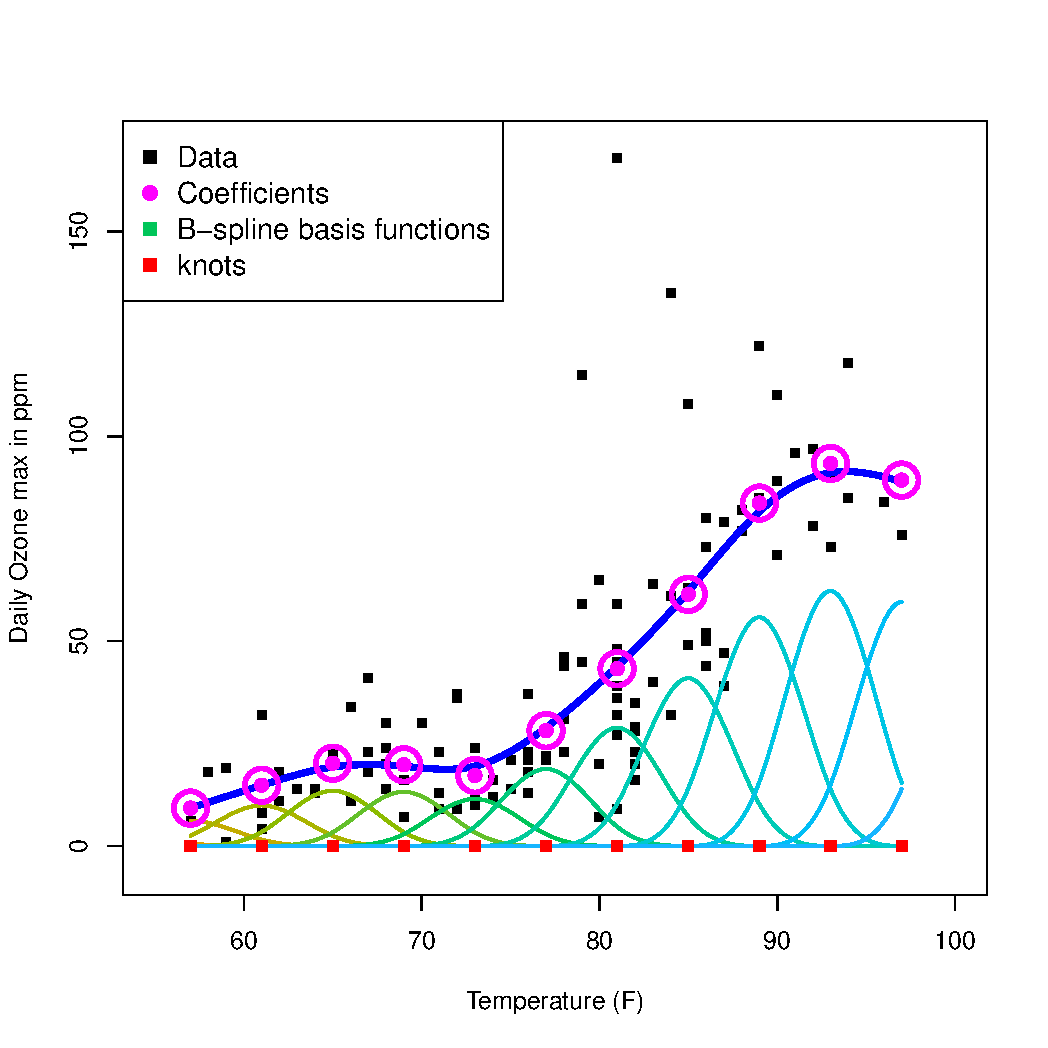
\includegraphics[width=.6\textwidth, height=.6\textheight,clip=true,trim = 0pt 15pt 0pt 10pt]{figures/fig3e}
\end{center}
}

\vfill

\vfill

\end{frame}


\begin{frame}[fragile]
 \frametitle{Penalized regression}
 	\framesubtitle{\quad P-splines (Eilers and Marx, 1996)}
 \vspace{.0cm}
{\footnotesize
\begin{itemize}
\item Estimation by \alert{penalized least squares}, such that:
\[
\mbox{min} \|\bfy - \bfB\bftheta\|^2  \rightarrow \hat{\bftheta} = (\bfB^\prime\bfB + \bfP )^{-1} \bfB^\prime \bfy  
\]
\vspace{-.4cm}
\[
\hat\bfy = \bfB \hat\bftheta
\]
\quad $\bfP$ is a \alert{roughness penalty for smoothness} controlled by $\lambda$ 
\medskip
\item Choose the size of $\bfB$ and $\lambda$ (and penalty order)
\begin{itemize}
\item $20<\mbox{knots}<40$
\item $\phantom{0}0 < \lambda < \infty$
\end{itemize}
\end{itemize}
}

\vfill

\vfill

\end{frame}


{\nologo
\begin{frame}[fragile]
 \frametitle{Penalized regression}
 	\framesubtitle{\quad P-splines (Eilers and Marx, 1996)}
 \vspace{.0cm}
{\footnotesize
\begin{itemize}
\item Choose $\lambda$ to tune the fit
\end{itemize}
}
 \vspace{-.3in}
\only<1>{
 \begin{center}
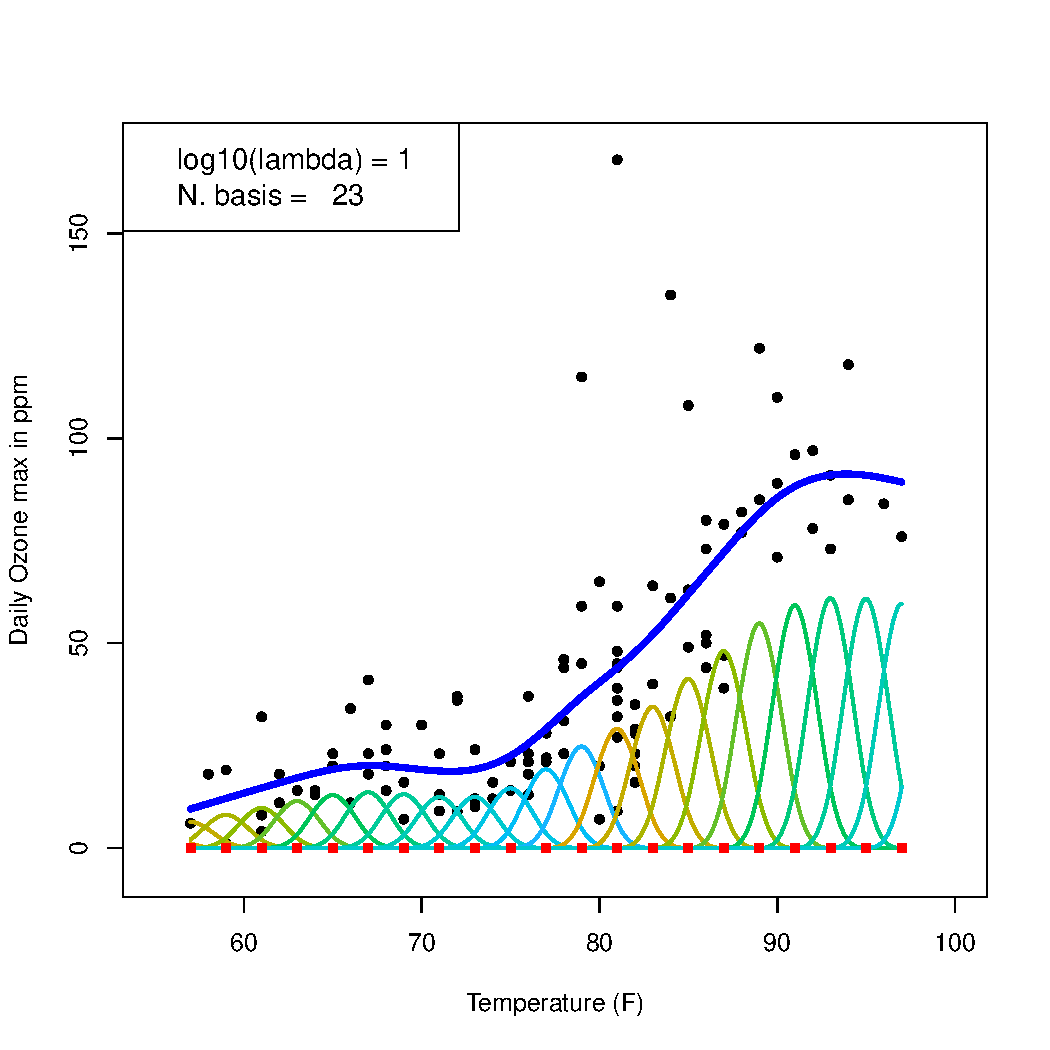
\includegraphics[width=.8\textwidth, height=.8\textheight,clip=true,trim = 0pt 15pt 0pt 10pt,page=1]{figures/a1a}
 \end{center}
}
\only<2>{
 \begin{center}
\includegraphics[width=.8\textwidth, height=.8\textheight,clip=true,trim = 0pt 15pt 0pt 10pt,page=84]{figures/a1a}
 \end{center}
}
\only<3>{
 \begin{center}
\includegraphics[width=.8\textwidth, height=.8\textheight,clip=true,trim = 0pt 15pt 0pt 10pt,page=14]{figures/a1b}
 \end{center}
}
\only<4>{
 \begin{center}
\includegraphics[width=.8\textwidth, height=.8\textheight,clip=true,trim = 0pt 15pt 0pt 10pt,page=27]{figures/a1b}
 \end{center}
}
\vfill

\vfill

\end{frame}
}


\begin{frame}
\frametitle{P-splines}
\framesubtitle{Knots and penalties}
 \footnotesize
 
 \begin{itemize}

 \item Choose a moderate number of equidistant knots ($k <<< n$), e.g. $20\leq k\leq 40$

 \item Add a penalty to the measure of fit, to tune smoothness 

 \begin{itemize}

 \item \footnotesize{Discrete differences of coefficients}
 \[
 \| \bfy - \bfB \bftheta \|^2 + {\color{red}\lambda \sum_j(\Delta^d \theta_j)^2}
 \]

\item[]\quad where $\Delta^d$ is a difference operator of order $d$, i.e.
\begin{align*}
 \Delta \bftheta_j &= \bftheta_{j} - \bftheta_{j-1} \tag{First order} \\
 \Delta^2 \bftheta_j &= \bftheta_{j} - 2 \bftheta_{j-1} + \bftheta_{j-2}  \tag{Second order} \\
 \vdots
\end{align*}
\end{itemize}
 \end{itemize}
 
 
\end{frame}
%


\begin{frame}
\frametitle{P-splines}
\framesubtitle{Penalties}

\footnotesize

\medskip

\begin{itemize}
  \item We are interested in differences on the coefficients 

  \item $\Delta^d\bftheta = \bfD_d\bftheta$ (\textit{Difference matrix operator}) 

\[
 \bfD_1 =\left[
\begin{array}{rrrrr}
- 1 &  1 &  0 & 0 & \cdots \cr
  0 & -1 &  1 & 0 & \cdots \cr
  0 &  0 & -1 & 1 & \cdots \cr
   \vdots & \vdots & \vdots & \vdots & \ddots
\end{array}\right]
\quad \mbox{or} \quad
\bfD_2 =\left[
\begin{array}{rrrrr}
 1 & -2 &  1 &  0 & \cdots\cr
 0 &  1 & -2 &  1 & \cdots\cr
 0 &  0 &  1 & -2 & \cdots\cr
 \vdots & \vdots & \vdots & \vdots & \ddots
\end{array}\right]
\]

 \item The \alert{penalty} becomes {$\bfP=\lambda\bfD^\prime\bfD$} \medskip
 
 \item Estimation is done by \alert{penalized least squares}:
 \[
 \min \|\bfy - \bfB\bftheta\|^2 + \bfP \rightarrow \hat{\bftheta}_{\lambda^*} = (\bfB^\prime\bfB + \bfP)^{-1}\bfB^\prime\bfy
 \]
 \item $\lambda^*$ can be selected by criteria as \alert{AIC}, \alert{BIC}, or \alert{GCV}

\end{itemize}

\vfill\vfill

\end{frame}





\begin{frame}[fragile]
\frametitle{Selection of $\lambda$}
 
 \footnotesize

\begin{itemize}
   \item Optimal $\lambda^*$ can be selected by criteria as \alert{AIC}, \alert{BIC}, or \alert{GCV}

\[
GCV=\sum_{i=1}^{n}\frac{(y_i-\hat y_i)^2}{n-trace(\bfH)}; \quad
\bfH=\bfB(\bfB^{\prime}\bfB+\lambda
\bfD^{\prime}\bfD)^{-1}\bfB^{\prime}\]
\[AIC=2log \left (\sum_{i=1}^{n} (y_i-\hat y_i)^2\right
)-2\log(n)+2\log\left ( trace(\bfH)\right ) 
\]
   \item Evaluate on a large grid of $\lambda$'s.
  

 \end{itemize}

\vfill
\vfill

\end{frame}



\begin{frame}[fragile]
\frametitle{Demo P-splines}
 \begin{itemize}
   \item \texttt{library(gamlss.demo)} 
   \item[] \quad \texttt{demoPsplines()}
 \end{itemize}
\end{frame}

%%%%%%%%%%%%%%%%%%%%%%%%%

\begin{frame}
 \frametitle{Smoothing and mixed models}
 	\framesubtitle{\quad a semi-parametric approach}
\footnotesize

 	\begin{itemize}
 	
 	\item Reformulate $\bfy= \bfB\bftheta + \bfepsilon$  into: 
 	
 	$$
 	  \bfy =  \bfX\bfbeta + \bfZ\bfalpha + \bfepsilon, \quad 
 	\begin{pmatrix}
 	\bfalpha \\
 	\bfepsilon
 	\end{pmatrix}
 	\sim
 	\mathcal{N}
 	\begin{bmatrix}
 	\begin{pmatrix}
 	0 \\
 	0
 	\end{pmatrix}
 	,
 	\begin{pmatrix}
 	   \bfG & \bfzero \\
 	\bfzero & \sigma^2\bfI
 	\end{pmatrix}
 	\end{bmatrix}
 	$$
 	
	\quad where $\bfG = \sigma^2_\alpha\bfI$, is the random effects covariance
 	
	\qquad \qquad $\lambda$ estimation becomes the ratio ${\sigma^2}/{\sigma_\alpha^2}$

 \item \alert{Flexibility:}
%
 \item[]\qquad$-$ Easy incorporation of smoothing in \alert{complex models}: hierarchical models, multi-level models, longitudinal data, correlated errors ...
% \medskip
%
 \item \alert{Mixed models theory} for {\bf estimation} and {\bf inference}
%
 \item \alert{Extension to non-gaussian data} (Poisson, Binomial, etc ...)
%
 \begin{itemize}
 \item \footnotesize Generalized Linear Models (GLM's) to GL(Mixed)M's
 \end{itemize}
 \end{itemize}
%%\pause

\vfill

\vfill


\end{frame}

{\nologo
\begin{frame}
 \frametitle{Bayesian P-splines}
 	\framesubtitle{Lang and Brezger (2004)}
\footnotesize

\begin{itemize}
 	\item The bayesian analogue of P-splines replace differences with Gaussian random walks as priors on the regression coefficients $\theta_j$
  \item First/second order 
 $\theta_j$, corresponds to a B-splines basis $\bfB$:
 \[\theta_j= \theta_{j-1}+v_j \quad \text{or}\quad \theta_j= 2\theta_{j-1}-\theta_{j-2}+v_j
  \]
  where  $v_j\sim N(0\tau^2)$
  \item The amount of smoothing is controlled by $\tau^2=\sigma^2/\lambda$
  \item In general, we can rewrite $\bfP$ as:
  \[
  \bftheta |\tau^2 \propto exp \left (-\frac{1}{2\tau^2} \bftheta^\prime \bfP
   \bftheta \right )
  \]
  the {\bf rank} of $\bfP$ is $c-1$ for fist order RW, and $c-2$ for 2nd order (improper prior)
\item As previously
$$
\bfy |\bftheta \sim N\left (\bfB \bftheta ,\bfI \sigma^2 \right ),
$$
\item Software \texttt{BayesX}, \texttt{Inla}
\item Hierarchical models (mixed model representation):  \texttt{BuGS}, \texttt{JAGS}
\end{itemize}
%%\pause

\end{frame}
}

%%%%%%%%%%%%%%%%%%%%%%%%

\begin{frame}[fragile]
\frametitle{Multidimensional P-splines}
 \footnotesize
 \begin{itemize}
   \item (Generalized) Additive Models (Hastie \& Tibshirani, 1990)
   $$
      \bfeta=f(\bfx_1)+f(\bfx_2)+ \bfepsilon
   $$
   \vspace{-.2in}
   \item Smooth ANOVA models (Lee and Durban, 2011)
   $$
      \bfeta=f(\bfx_1)+f(\bfx_2)+f(\bfx_1,\bfx_2)  + \bfepsilon
   $$
   \vspace{-.2in}
   \item For higher dimensions one may incur in the {\bf curse of dimensionality} (computational problems)
   
   \item Other approaches includes Thin plate splines (radial basis functions). Problems: knots selection and position in larger dimensions.
   
   \item Recommended approach use for interactions: \alert{Tensor Products}
 \end{itemize}
 
 \vfill
 
 \vfill
 
\end{frame}

%%%%%%%%%%%%%%%%%%%%%%%%%


\begin{frame}[fragile]
\frametitle{GAMs with P-splines}
 \footnotesize
 \begin{itemize}
   \item Use B-splines $\bfeta = f(x_1 + f(x_2) = B_1\theta_1 + B_2 \theta_2$
   \item Vectorize and combine
    $$
       \bfeta =  [ B_1 : B_2 ] 
       \begin{bmatrix}
        \theta_1 \\
        \theta_2
       \end{bmatrix}
       =  \bfB \bftheta
    $$
    \item Difference penalty is blockdiagonal, i.e. 
    $$
    \bfP = \mbox{bdiag}(\bfP_1,\bfP_2) = 
     \begin{bmatrix}
        \lambda_1 D_1^\prime D_1 &      \\
                                 & \lambda_2 D_2^\prime D_2
     \end{bmatrix}
    $$
   \item In general $\lambda_1 \neq \lambda_2$ (Anisotopic smoothing)
 \end{itemize}
 
 \vfill
 
 \vfill
 
\end{frame}


\begin{frame}[fragile]
\frametitle{Two-dimensional smoothing with P-splines}
 \footnotesize
 \begin{itemize}
   \item Use B-splines $\bfeta = f(x_1 + f(x_2) = B_1\theta_1 + B_2 \theta_2$
   \item Vectorize and combine
    $$
       \bfeta =  [ B_1 : B_2 ] 
       \begin{bmatrix}
        \theta_1 \\
        \theta_2
       \end{bmatrix}
       =  \bfB \bftheta
    $$
    \item Difference penalty is blockdiagonal, i.e. 
    $$
    \bfP = \mbox{bdiag}(\bfP_1,\bfP_2) = 
     \begin{bmatrix}
        \lambda_1 D_1^\prime D_1 &      \\
                                 & \lambda_2 D_2^\prime D_2
     \end{bmatrix}
    $$
   \item In general $\lambda_1 \neq \lambda_2$ (Anisotopic smoothing)
 \end{itemize}
 
 \vfill
 
 \vfill
 
\end{frame}


{\nologo
\begin{frame}
 \frametitle{$2d$ P-splines}
 	\framesubtitle{Bivariate smoothing}
 \vspace{-.10cm}
{\scriptsize
\begin{itemize}
\item Bivariate data, $(\bfx_1,\bfx_2,\bfy)$, regression model $\mbox{E}[\bfy|\bfx_1,\bfx_2] = f(\bfx_1,\bfx_2)$ %\medskip

\item $B$-splines on $\bfx_1$ and $\bfx_2$ domains, i.e. $B_k(x_1)$ and $B_l(x_2)$ %medskip

\item We aim to build a {\bf surface} as a \alert{sum of Tensor products} 
\vspace{-.1cm}
\[
f(\bfx_1,\bfx_2) = \sum_k \sum_l B_k(x_1) B_l(x_2) \theta_{kl}
\]\vspace{-.5cm}
\item Now we have a matrix of coefficients $\bfA=[\theta_{kl}]$, to be penalized with $\lambda_1$ and $\lambda_2$
\end{itemize}
}
%
\vspace{-.0cm}

{\footnotesize
{\bf E.g.:} Air quality data in NYC

\begin{minipage}[c]{.55\columnwidth}
\vspace{-.55in}
\begin{itemize}
\item Covariates: 
\begin{itemize}
\item \scriptsize$\bfx_1 = $ Daily max temperature (in F)
\item \scriptsize$\bfx_2 = $ Wind speed (in mph)
\end{itemize}
\vfill
\vfill

\end{itemize}
\end{minipage}
\begin{minipage}[c]{.4\columnwidth}
\begin{center}
\only<1>{
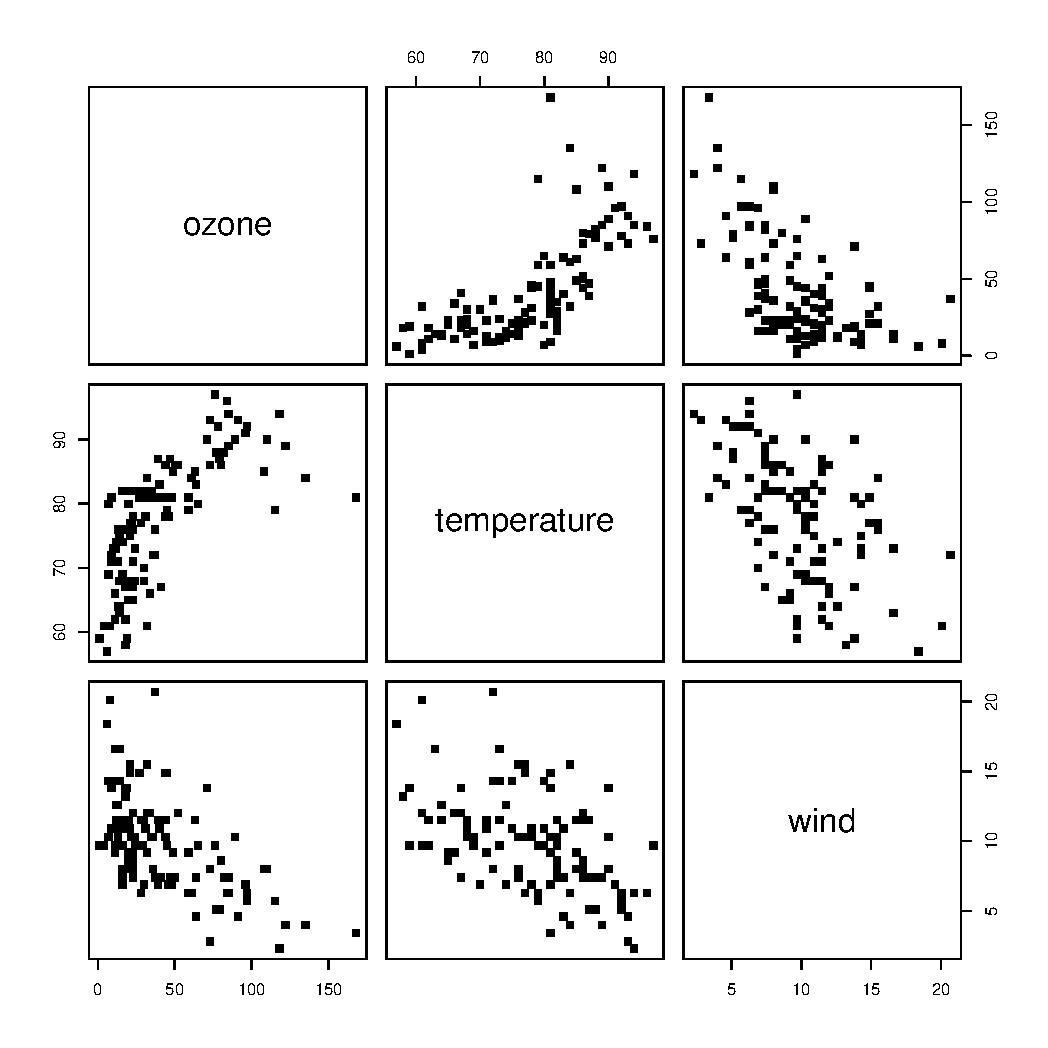
\includegraphics[width=3.5cm,height=3.25cm]{figures/fig4} }
\only<2>{
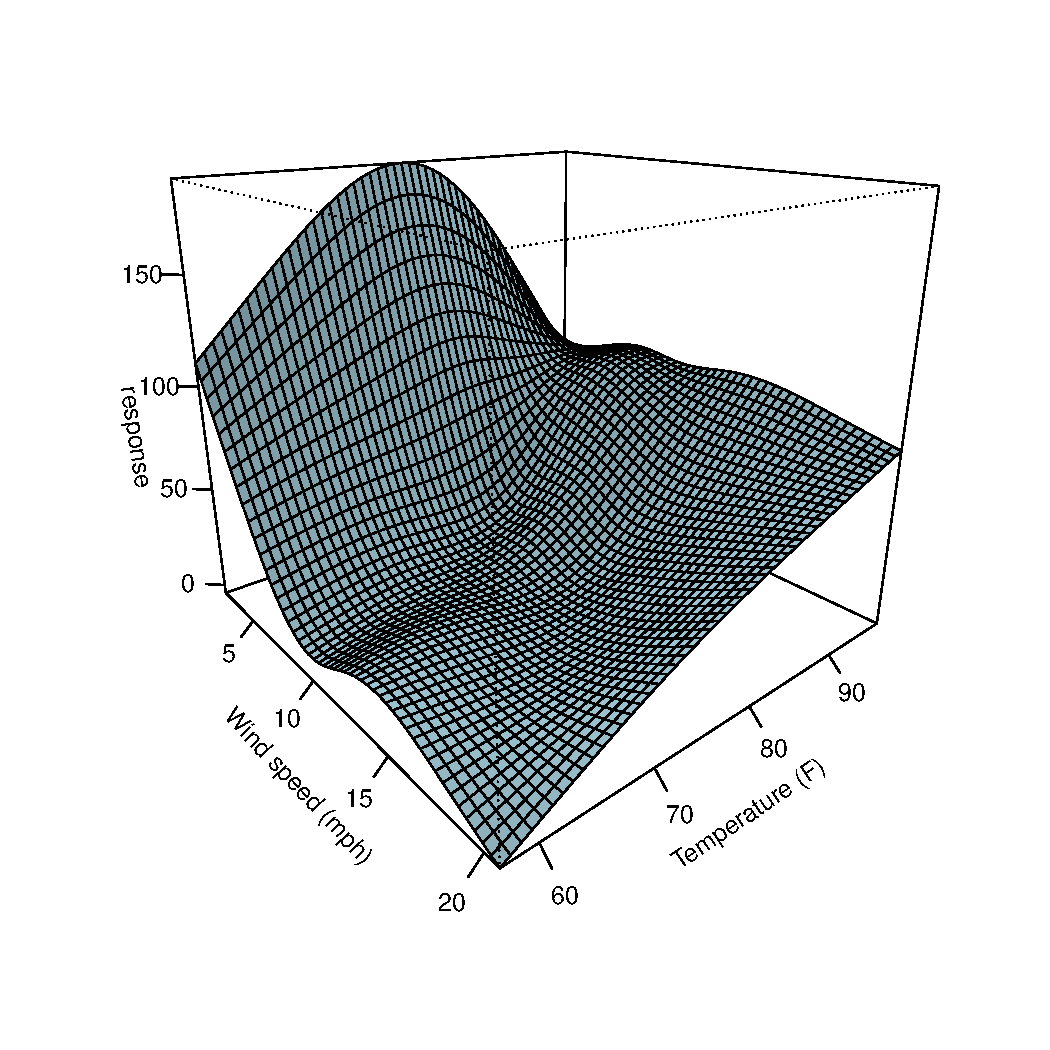
\includegraphics[width=3.5cm,height=3.25cm]{figures/fig5} }
\end{center}
\end{minipage}
}

\end{frame}
}


%%%%%%%%%%%%%%%%%%%%%%%%%%%%


{\nologo
\begin{frame}
	\frametitle{Multidimensional smoothing}
		\framesubtitle{\quad Array structured data}
	\vspace{.08in}	
	
\footnotesize

\medskip

\begin{minipage}[c]{.45\columnwidth}

\begin{itemize}
\item \alert{Data} $\bfY= \bfy_{ij}$, {\tiny $i=1,...,n_1$ and $j=1,...,n_2$}

\item \alert{Array structure}: $n_1$ rows and $n_2$ columns
\[
\bfY = 
 \left[
\begin{array}{cccc}
 y_{11} &  y_{12} & \cdots & y_{1{}n_2} \crcr
 y_{21} &  y_{22} & \cdots & y_{2{}n_2} \crcr
 \vdots    &  \vdots    & \ddots & \vdots    \crcr
 y_{n_{1}1} &  \cdots & \cdots & y_{n_{1}n_{2}} 
\end{array}
 \right]
\]
\vspace{-0.3cm}
\item {\bf Regressors:}
\begin{align*}
 \bfx_1 &= (x_{1{}1},\cdots,x_{1{n_1}})^\prime \cr
 \bfx_2 &= (x_{2{}1},\cdots,x_{2{}n_2})^\prime
\end{align*}
\vspace{-0.3cm}
\end{itemize}
\end{minipage}
\hfill{}
\begin{minipage}[c]{.5\columnwidth}
\begin{center}
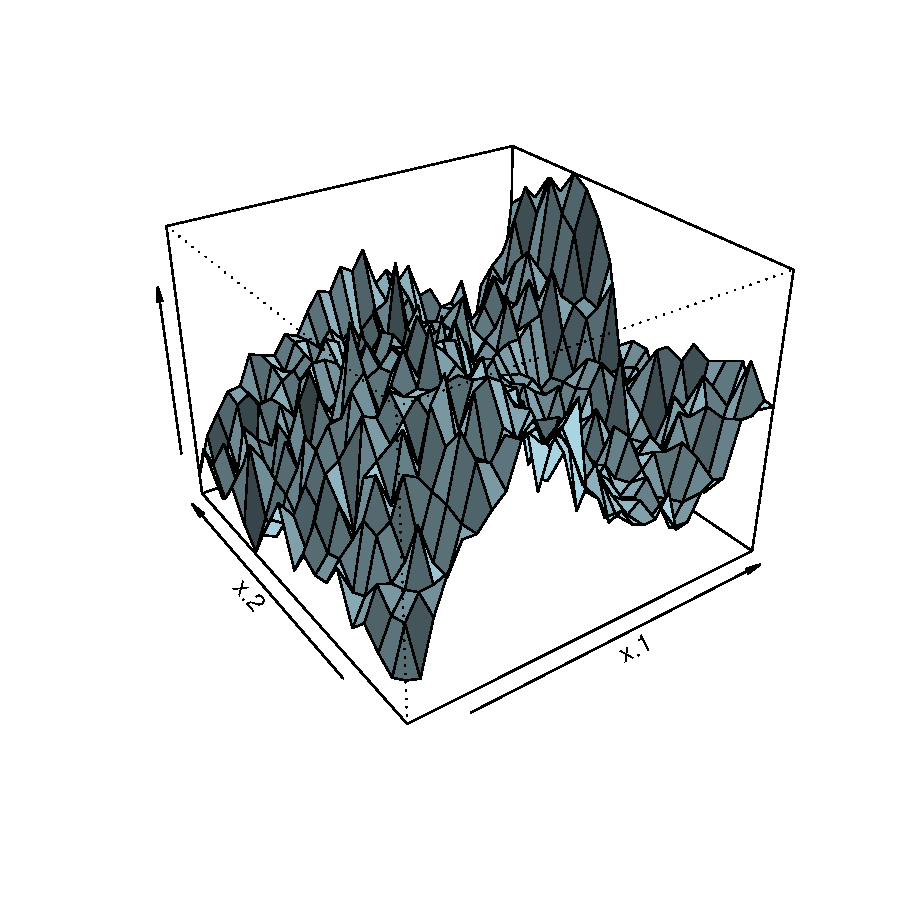
\includegraphics[width=5.5cm,height=4.5cm]{figures/EX_2dmixed_data}
\end{center}
\end{minipage}
\begin{itemize}
\item \textbf{e.g.:} image data, mortality life tables, micro-arrays etc ... 
\end{itemize}
\end{frame}
}



{\nologo
\begin{frame}
	\frametitle{Multidimensional smoothing}
	\framesubtitle{\quad Array structured data}
	\vspace{.05in}

\begin{minipage}[c]{.45\columnwidth}
\footnotesize{
$-$ \alert{Tensor Products of $B$-splines} \medskip
\begin{itemize}
  \item {\bf Marginal Basis:}
\begin{itemize}
\item $\bfB_1 = \bfB_1(\bfx_1)$, $n_1 \times c_1$
\item $\bfB_2 = \bfB_2(\bfx_2)$, $n_2 \times c_2$
\end{itemize}

 \item \alert{$2d$ $B$-splines Basis:}
\begin{itemize}
\item Kronecker Product ($\bfotimes$) of marginal basis:
$$\bfB = \bfB_2 \bfotimes \bfB_1,\quad n_1{}n_2 \times c_1{}c_2$$
\end{itemize}
\vspace{-.3cm}
  \item Computationally efficient methods \alert{(GLAM, Currie, Durban and Eilers, 2006)}
\end{itemize}
}
\end{minipage}
\hfill{}
\begin{minipage}[c]{.45\columnwidth}
\begin{tabular}{c}
\mbox{\scriptsize Tensor product of $2$ cubic $B$-splines} \\
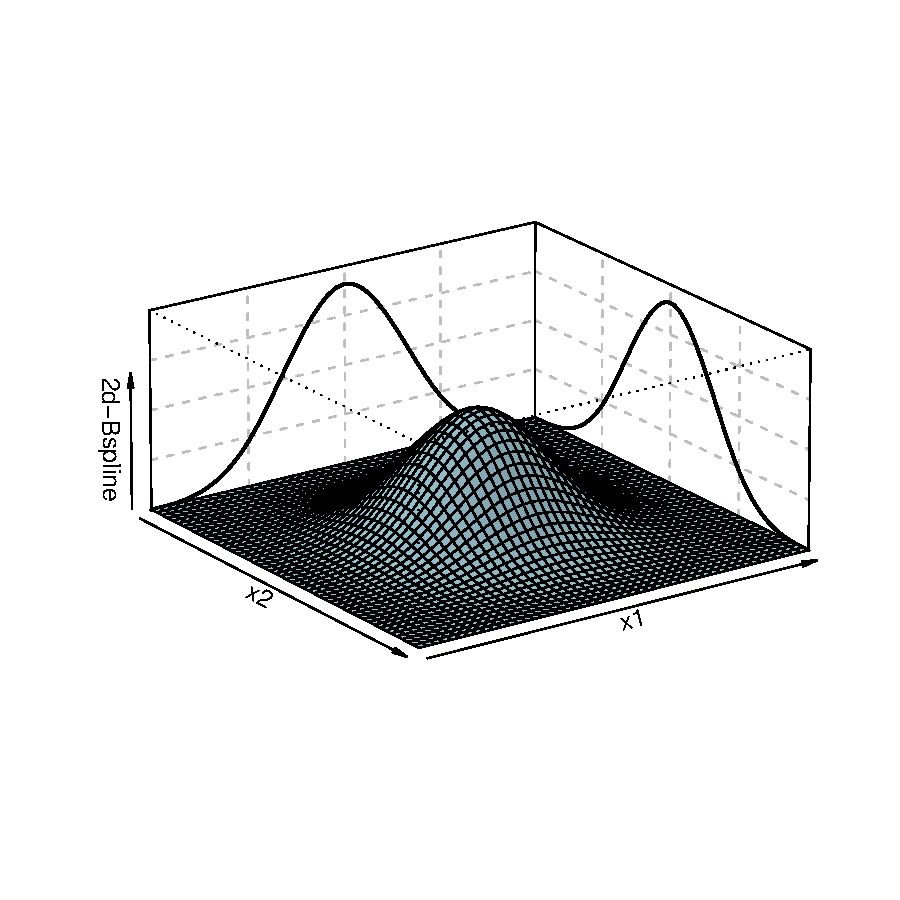
\includegraphics[width=4.cm,height=3.cm]{figures/EX_2dBsplines1} \\
\mbox{\scriptsize $B$-spline basis of $3\times 3$} \\
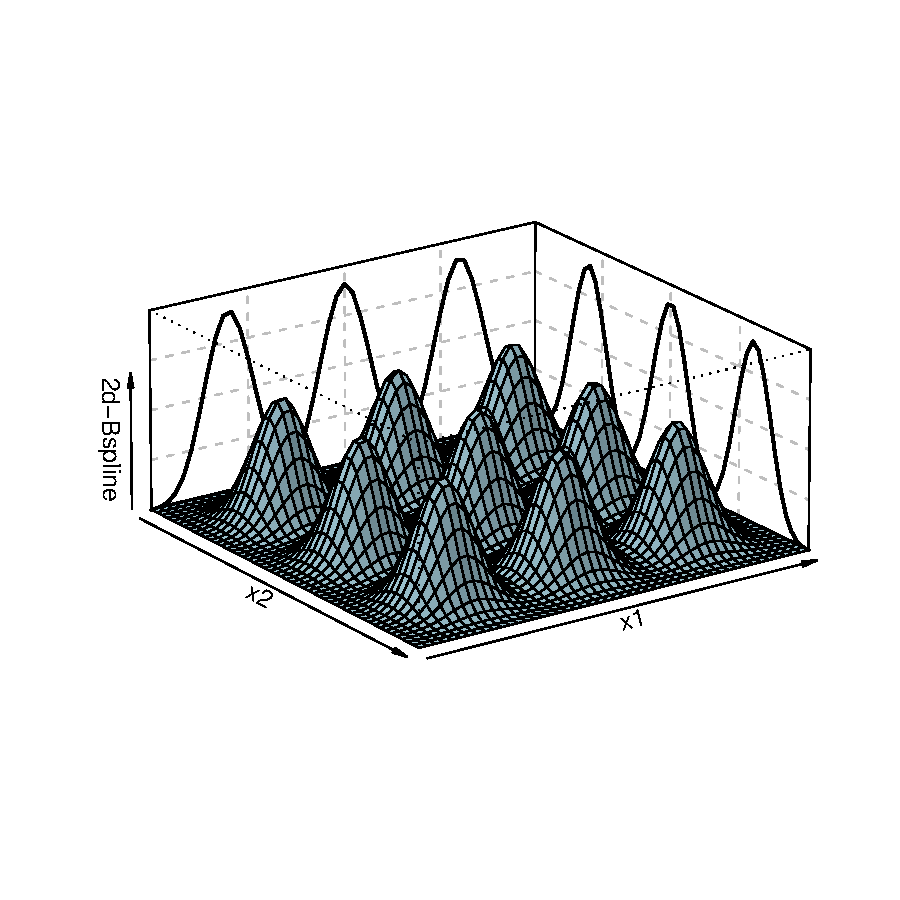
\includegraphics[width=4.cm,height=3.cm]{figures/EX_2dBsplines3}
\end{tabular}
\end{minipage}

%\vspace{-1.5cm}
% {\tiny\color{LightBlue}>> P-spline fit}
\end{frame}
%
}


{\nologo
\begin{frame}[fragile]
\frametitle{References}

\footnotesize

\begin{thebibliography}{9}
\setbeamertemplate{bibliography item}[book]
 \bibitem{Hastie90}
Hastie T.J. and Tibshirani, R.J. (1990)
\newblock{\em Generalized Additive Models}
\newblock Chapman & Hall/CRC Monographs on Statistics & Applied Probability

\setbeamertemplate{bibliography item}[article]
 \bibitem{Eilers96}
Eilers P.H.C., and Marx B.D. (1996)
\newblock{\em Flexible Smoothing with B-splines and Penalties}
\newblock Statistical Science, Vol. 11, No. 2., pp. 89-102

\setbeamertemplate{bibliography item}[article]
 \bibitem{Lang04}
     Lang, S. and Brezger, A.
\newblock {\em Bayesian P-Splines}
\newblock Journal of Computational and Graphical Statistics. Vol 13, 2004, pages 183-212

\setbeamertemplate{bibliography item}[article]
 \bibitem{Lee11}
 Lee, D.-J. and Durb\'an, M. (2011)
 \newblock{\em P-spline ANOVA-type interaction models for spatio-temporal smoothing}
 \newblock Statistical Modelling, Vol. 11, Issue 1, Pages 49-69.

\setbeamertemplate{bibliography item}[article]
 \bibitem{Lee11}
 Ruppert, D., Wand, M.P. and Carroll, R.J. (2009)
 \newblock{\em Semiparametric regression during 2003–2007}
 \newblock Electron. J. Statist. Volume 3 (2009), 1193-1256.
 
 \setbeamertemplate{bibliography item}[article]
   \bibitem{Currie06}
     Currie, ID., Durb\'an M. and Eilers, PHC. (2006)
\newblock {\em Generalized linear array models with
applications to multidimensional smoothing}
\newblock JRSSB, 68:1-22

   \end{thebibliography}

\vfill

\vfill

\end{frame}



\section{Penalized splines in {\bf R}}


\begin{frame}[fragile]
\frametitle{Penalized splines in \texttt{R}}
 \framesubtitle{What's next?}


\begin{center}
 \url{http://idaejin.github.io/bcam-courses/jjseb3/R-jjseb3.html}
\end{center}

\end{frame}
}



\end{document}



% 
 <<>>=
  #library(knitr)
  #Stangle("BCAM-Course-GLM.Rnw",output="BCAM-Course-GLM.R")
 @
